
In the previous section, we learned how AST is represented in Clang and learned what its in-memory classes look like. We also learned about some useful skills we can use to perform pattern matching on Clang AST. In this section, we will learn how to write plugins that allow you to insert custom AST processing logic into Clang's compilation pipeline.

This section will be divided into three parts:

\begin{itemize}
\item Project overview: The goal and overview of the demo project we are going to create in this section.

\item Printing diagnostic messages: Before we dive into the core of developing a plugin, we are going to learn how to use Clang's DiagnosticsEngine, a powerful subsystem that helps you print out well-formatted and meaningful diagnostic messages. This will make our demo project more applicable to real-world scenarios.

\item Creating the AST plugin: This section will show you how to create an AST plugin from scratch, fill in all the implementation details, and how to run it with Clang.
\end{itemize}

\subsubsubsection{7.3.1\hspace{0.2cm}Project overview}

In this section, we will create a plugin that prompts the user with warning messages whenever there are if-else statements in the input code that can be converted into ternary operators.

\begin{tcolorbox}[colback=blue!5!white,colframe=blue!75!black, fonttitle=\bfseries,title=Quick Refresher – Ternary Operator]
\hspace*{0.7cm}The ternary operator, x? val\_1 : val\_2, is evaluated to val\_1 when the x condition is true. Otherwise, it is evaluated to val\_2.
\end{tcolorbox}

For example, let's look at the following C/C++ snippet:

\begin{lstlisting}[style=styleCXX]
int foo(int c) {
	if (c > 10) {
		return c + 100;
	} else {
		return 94;
	}
}

void bar(int x) {
	int a;
	if (x > 10) {
		a = 87;
	} else {
		a = x – 100;
	}
}
\end{lstlisting}

The if-else statements in both functions can be converted into ternary operators, like this:

\begin{lstlisting}[style=styleCXX]
int foo(int c) {
	return c > 10? c + 100 : 94;
}

void bar(int x) {
	int a;
	a = x > 10? 87 : x – 100;
}
\end{lstlisting}

In this project, we will only focus on finding two kinds of potential ternary operator opportunities:

\begin{itemize}
\item Both the then block (true branch) and the else block (false branch) contain a single return statement. In this case, we can coalesce their return values and the branch condition into one ternary operator (as the new returned value).

\item Both the then block and the else block only contain a single assignment statement. Both statements use a single DeclRefExpr – that is, a symbol reference – as the LHS, and both DeclRefExpr objects point to the same Decl (symbol). In other words, we are covering the case of the bar function shown in the preceding snippet. Note that we are not covering cases where the LHS is more complicated; for example, where an array subscription, a[i], is used as the LHS.
\end{itemize}

After identifying these patterns, we must prompt warning messages to the user and provide extra information to help the user fix this issue:

\begin{tcblisting}{commandshell={}}
$ clang …(flags to run the plugin) ./test.c
./test.c:2:3: warning: this if statement can be converted to ternary operator:
  if (c > 10) {
  ^
./test.c:3:12: note: with true expression being this:
    return c + 100;
            ^
./test.c:5:12: note: with false expression being this:
    return 94;
            ^
./test.c:11:3: warning: this if statement can be converted to ternary operator:
  if (x > 10) {
  ^
./test.c:12:9: note: with true expression being this:
    a = 87;
         ^
./test.c:14:9: note: with false expression being this:
    a = x - 100;
         ^
2 warnings generated.
\end{tcblisting}

Each warning message – which tells you which if-else statement can be converted into a ternary operator – is followed by two notes pointing out the potential expressions to construct for the operator.

Compared to handcrafting compiler messages, as we did in the Developing custom preprocessor plugins and callbacks section of Chapter 6, Extending the Preprocessor, here, we are using Clang's diagnostics infrastructure to print messages that carry richer information, such as the snapshot of code that the message is referring to. We will show you how to use that diagnostic infrastructure next.

\subsubsubsection{7.3.2\hspace{0.2cm}Printing diagnostic messages}

In Chapter 6, Extending the Preprocessor, we asked if you could improve the warning message format in the example project shown in the Developing custom preprocessor plugins and callbacks section, so that it's closer to the compiler messages you saw from Clang. One of the solutions to that question is using Clang's diagnostic framework. We are going to look at this in this section.

Clang's diagnostic framework consists of three primary parts:

\begin{itemize}
\item Diagnostic IDs
\item Diagnostic engine
\item Diagnostic consumers (clients)
\end{itemize}

Their relationships can be seen in the following diagram:

\hspace*{\fill} \\ %插入空行
\begin{center}
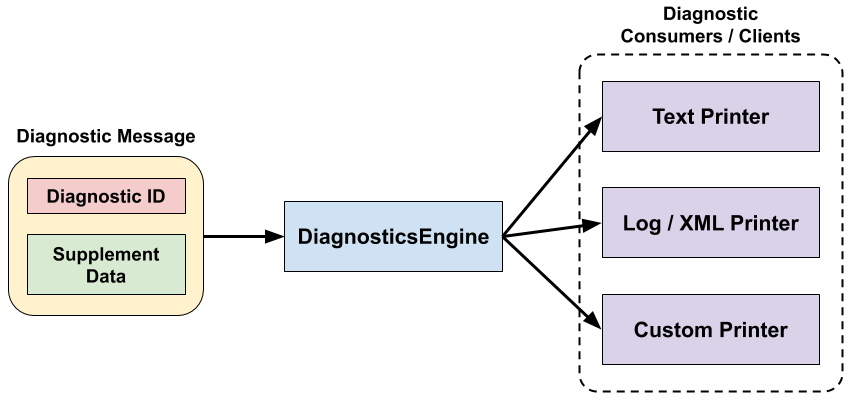
\includegraphics[width=0.9\textwidth]{content/2/chapter7/images/5.png}\\
Figure 7.5 – High-level organization of Clang's diagnostic framework
\end{center}

\hspace*{\fill} \\ %插入空行
\noindent
\textbf{Diagnostic messages}

Starting from the left-hand side of the preceding diagram, most of the time, a diagnostic message – for example, use of undeclared identifier "x" – is associated with a message template that has its own diagnostic ID. Using the undeclared identifier message, for example, its message template looks like this:

\begin{tcblisting}{commandshell={}}
"use of undeclared identifier %0"
\end{tcblisting}

\%0 is a placeholder that will be filled in by supplemental data later. In this case, it is the concrete identifier name (x, in the preceding example message). The number following \% also suggests which supplemental data it will use. We will cover this format in detail shortly.

Templates are registered with the diagnostic engine via TableGen syntax. For example, the message we are discussing here is put inside clang/include/clang/Basic/DiagnosticSemaKinds.td:

\begin{lstlisting}[style=stylePython]
def err_undeclared_var_use : Error<"use of undeclared identifier %0">;
\end{lstlisting}

We highlighted two parts in the preceding snippet. First, the name of this message template, err\_undeclared\_var\_use, will be used later as the unique diagnostic ID. Second, the Error TableGen class suggested that this is an error message, or more formally speaking, its diagnostic level error.

In summary, a diagnostic message consists of a unique diagnostic ID – which is associated with a message template and its diagnostic level – and the supplemental data to put in the placeholders of the template, if there are any.

\hspace*{\fill} \\ %插入空行
\noindent
\textbf{Diagnostic consumers}

After the diagnostic message is sent to the diagnostic engine – represented by the DiagnosticsEngine class – the engine formats the messages into textual contents and send them to one of the diagnostic consumers (also called clients in the code base; we will use the term consumer in rest of this section).

A diagnostic consumer – an implementation of the DiagnosticConsumer class – post-processes the textual messages sent from DiagnosticsEngine and exports them via different mediums. For example, the default TextDiagnosticPrinter prints messages to the command-line interface; LogDiagnosticPrinter, on the other hand, decorates the incoming messages with simple XML tags before printing them into log files. In theory, you can even create a custom DiagnosticConsumer that sends diagnostic messages to a remote host!

\hspace*{\fill} \\ %插入空行
\noindent
\textbf{Reporting diagnostic messages}

Now that you have learned how Clang's diagnostic framework works, let's learn how to send (report) a diagnostic message to DiagnosticEngine:

\begin{enumerate}
\item First, we need to retrieve a reference to DiagnosticEngine. The engine itself is sitting at the core of Clang's compilation pipeline, so you can fetch it from various primary components, such as ASTContext and SourceManager. The following is an example:

\begin{lstlisting}[style=styleJavaScript]
// `Ctx` has the type of `ASTContext&`
DiagnosticsEngine& Diag = Ctx.getDiagnostics();
\end{lstlisting}

\item Next, we need to use the DiagnosticsEngine::Report function. This function always takes a diagnostic ID as one of its arguments. For example, to report err\_undeclared\_var\_use, which we introduced earlier, use the following code:

\begin{lstlisting}[style=styleJavaScript]
Diag.Report(diag::err_undeclared_var_use);
\end{lstlisting}

However, we know that err\_undeclared\_var\_use takes one placeholder argument – namely, the identifier name – which is supplied through concatenating the Report function call with << operators:

\begin{lstlisting}[style=styleJavaScript]
Diag.Report(diag::err_undeclared_var_use) << ident_name_str;
\end{lstlisting}

\item Recall that err\_undeclared\_var\_use only has one placeholder, \%0, so it picks up the first values in the following << stream. Let's say we have a diagnostic message, err\_invalid\_placement, with the following template:

\begin{lstlisting}[style=styleJavaScript]
"you cannot put %1 into %0"
\end{lstlisting}

\item You can report this using the following code:
\begin{lstlisting}[style=styleJavaScript]
Diag.Report(diag::err_invalid_placement)
            << "boiling oil" << "water";
\end{lstlisting}


\item In addition to simple placeholders, another useful feature is the \%select directive. For example, we have a diagnostic message, warn\_exceed\_limit, with a template like this:

\begin{lstlisting}[style=styleJavaScript]
"you exceed the daily %select{wifi|cellular network}0 limit"
\end{lstlisting}

The \%select directive consists of curly braces in which different message options are separated by |. Outside the curly braces, a number – 0, in the preceding code – indicates which supplement data is used to select the option within the braces. The following is an example of this:

\begin{lstlisting}[style=styleJavaScript]
Diag.Report(diag::warn_exceed_limit) << 1;
\end{lstlisting}

The preceding snippet will output You exceed the daily cellular network limit. Let's say you use 0 as the parameter after the stream operator (<<):

\begin{lstlisting}[style=styleJavaScript]
Diag.Report(diag::warn_exceed_limit) << 0;
\end{lstlisting}

This will result in a message stating you exceed the daily wifi limit.

\item Now, let's say you use another version of the Report function, which takes an additional SourceLocation argument:

\begin{lstlisting}[style=styleJavaScript]
// `SLoc` has the type of `SourceLocation`
Diag.Report(SLoc, diag::err_undeclared_var_use)
                  << ident_name_str;
\end{lstlisting}

The output message will contain part of the source code being pointed to by SLoc:

\begin{tcblisting}{commandshell={}}
test.cc:2:10: error: use of undeclared identifier 'x'
  return x + 1;
          ^
\end{tcblisting}

\item Last but not least, though most of the diagnostic messages are registered with DiagnosticsEngine via TableGen code put inside Clang's source tree, this doesn't mean that developers cannot create their new diagnostic messages without modifying Clang's source tree. Let's introduce DiagnosticsEngine::getCustomDiagID(…), the API that creates a new diagnostic ID from a message template and diagnostic level provided by developers:

\begin{lstlisting}[style=styleJavaScript]
auto MyDiagID = Diag.
getCustomDiagID(DiagnosticsEngine::Note,
"Today's weather is %0");
\end{lstlisting}

The preceding snippet creates a new diagnostic ID, MyDiagID, that has a message template of Today's weather is \%0 at its note diagnostic level. You can use this diagnostic ID just like any other ID:

\begin{lstlisting}[style=styleJavaScript]
Diag.Report(MyDiagID) << "cloudy";
\end{lstlisting}

\end{enumerate}

In this section, you learned how to leverage Clang's diagnostic framework to print out messages just like normal compiler messages.

Next, we are going to combine all the skills we've learned about in this chapter to create a custom AST plugin.

\subsubsubsection{7.3.3\hspace{0.2cm}Creating the AST plugin}

In the previous sections of this chapter, we explored Clang's AST and learned how to use it in in-memory APIs. In this section, we will learn how to write a plugin that helps you insert your custom AST processing logic into Clang's compilation pipeline in an easy way.

In Chapter 5, Exploring Clang's Architecture, we learned about the advantages of using Clang (AST) plugins: they can be developed even you are using a prebuilt clang executable, they are easy to write, and they have good integration with the existing toolchain and build systems, to name a few. In Chapter 6, Extending the Preprocessor, we developed a plugin for custom pragma handling in the preprocessor. In this chapter, we will also be writing a plugin, but this one will be designed for custom AST processing. The code skeletons for these two plugins are also quite different.

We introduced the sample project we will be using in this section in the Project overview section. This plugin will prompt users with warning messages if some if-else statements in the input code can be converted into ternary operators. In addition, it also shows extra hints about candidate expressions for building the ternary operator.

Here are the detailed steps for building the plugin:

\begin{enumerate}
\item Similar to the pragma plugin we saw in Chapter 6, Extending the Preprocessor, creating a plugin in Clang is basically like implementing a class. In the case of the AST plugin, this will be the PluginASTAction class.

PluginASTAction is a subclass of ASTFrontendAction – a FrontendAction specialized for handling AST (if you're not familiar with FrontendAction, feel free to read Chapter 5, Exploring Clang's Architecture, again). Thus, we need to implement the CreateASTConsumer member function:
\begin{lstlisting}[style=styleCXX]
struct TernaryConverterAction : public PluginASTAction {
	std::unique_ptr<ASTConsumer>
	CreateASTConsumer(CompilerInstance &CI,
                      StringRef InFile) override;
};
\end{lstlisting}
We will fill in this function later.


\item In addition to CreateASTConsumer, there are two other member functions we can override to change some of the functionalities: getActionType and ParseArgs. The former tells Clang how this plugin should be executed by returning one of the enum values shown here:

\begin{enumerate}[label=\alph*.]
\item Cmdline: The plugin will be executed after the main action if users provide the -plugin <plugin name> (frontend) command-line flag.

\item ReplaceAction: This replaces the original action Clang was going to perform. For example, if Clang was supposed to compile input code into an object file (the -c flag), it will execute the plugin's action instead once the plugin has been loaded.

\item AddBefore/AfterMainAction: The original Clang action will still be executed, and the plugin action will be prepended/appended to it.
\end{enumerate}

Here, we will use the Cmdline action type:

\begin{lstlisting}[style=styleCXX]
struct TernaryConverterAction : public PluginASTAction {
	…
	ActionType getActionType() override { return Cmdline; }
};
\end{lstlisting}

The ParseArgs member function, on the other hand, handles (frontend) command-line options specific to this plugin. In other words, you can create custom command-line flags for your plugin. In our case, we are going to create two flags: -no-detect-return and -no-detect-assignment. This allows us to decide whether we wish to detect potential ternary conversions regarding return statements or assignment statements, respectively:

\begin{lstlisting}[style=styleCXX]
struct TernaryConverterAction : public PluginASTAction {
	…
	bool NoAssignment = false,
	NoReturn = false;
	bool ParseArgs(const CompilerInstance &CI,
	const std::vector<std::string> &Args) override {
		for (const auto &Arg : Args) {
			if (Arg == "-no-detect-assignment") NoAssignment =
			true;
			if (Arg == "-no-detect-return") NoReturn = true;
		}
	    return true;
    }
};
\end{lstlisting}

As shown in the preceding snippet, we created two boolean flags, NoReturn and NoAssignment, to carry our command-line options' values. An important thing to know is the return value for ParseArgs. Instead of returning if it parsed any custom flag, ParseArgs is actually returning if the plugin should continue its execution. Therefore, you should always return true in most cases.

\item Now, we are going to talk about the content of CreateASTConsumer. This function will return an ASTConsumer object, which is the main body that we will put our custom logic in. Nevertheless, we are not going to directly implement an ASTConsumer. Instead, we are going to us the ASTConsumer object that was generated by ASTMatcher, which we introduced earlier in this chapter.

Recall that two things are required to build a MatchFinder instance – the primary pattern matching driver in ASTMatcher (patterns written in ASTMatcher's own DSL) and a MatchCallback implementation. Let's separate our patterns and matcher callbacks into two categories: patterns for detecting potential ternary operator opportunities based on return statements and those for detecting assignment-statement-based opportunities.

Here is the skeleton for CreateASTConsumer:

\begin{lstlisting}[style=styleCXX]
using namespace ast_matchers;
struct TernaryConverterAction : public PluginASTAction {
	…
private:
	std::unique_ptr<MatchFinder> ASTFinder;
	std::unique_ptr<MatchFinder::MatchCallback>
	  ReturnMatchCB, AssignMatchCB;
};

std::unique_ptr<ASTConsumer>
TernaryConverterAction::CreateASTConsumer
(CompilerInstance &CI, StringRef InFile) {
	ASTFinder = std::make_unique<MatchFinder>();
	// Return matcher
	if (!NoReturn) {
		ReturnMatchCB = /*TODO: Build MatcherCallback
		instance*/
		ASTFinder->addMatcher(traverse
		  (TK_IgnoreUnlessSpelledInSource,
		    /*TODO: Patterns in DSL*/), ReturnMatchCB.get());
	}
	// Assignment matcher
	if (!NoAssignment) {
		AssignMatchCB = /*TODO: Build MatcherCallback
		  instance*/
		ASTFinder->addMatcher(traverse
		  (TK_IgnoreUnlessSpelledInSource,
		    /*TODO: Patterns in DSL*/), AssignMatchCB.get());
	}
	return std::move(ASTFinder->newASTConsumer());
}
\end{lstlisting}

The preceding code created three additional unique\_ptr type member variables: one for holding MatchFinder and two MatchCallback ones for return-based and assignment-based patterns.

\begin{tcolorbox}[colback=blue!5!white,colframe=blue!75!black, fonttitle=\bfseries,title=Why Use unique\_ptr?]	\hspace*{0.7cm}The rationale behind using unique\_ptr to store those three objects – or storing those objects persistently – is because the ASTConsumer instance we created at the end of CreateASTConsumer (ASTFinder->newASTConsumer()) keeps references to those three objects. Thus, we need a way to keep them alive during the lifetime of the frontend.
\end{tcolorbox}

In addition to that, we registered the pattern for traversal with MatchFinder by using MatchFinder::addMatcher, the traverse function, and MatchCallback instances. If you're not familiar with these APIs, feel free to check out the ASTMatcher section.

Now, we only need to compose the matching patterns and implement some callbacks to print out warning messages if there is a match – as the TODO comments suggested in the preceding snippet.

\item Let's deal with the patterns first. The patterns we are looking for – both return-based and assignment-based patterns – have if-else statements (IfStmt) enclosed by a function (FunctionDecl for the entire function and CompoundStmt for the function body) in their outermost layout. Inside both, in the true branch and false branch of IfStmt, only one statement can exist. This structure can be illustrated like so:

\begin{tcolorbox}[colback=white,colframe=black]
\tt
\zihao{-5}
FunctionDecl \\
\hspace*{0.3cm}|\_CompoundStmt \\
\hspace*{0.6cm}|\_(Other AST nodes we don't care) \\
\hspace*{0.6cm}|\_IfStmt \\
\hspace*{0.9cm}|\_(true branch: contain only one return/assign statement) \\
\hspace*{0.9cm}|\_(false branch: contain only one return/assign statement)
\end{tcolorbox}

To convert this concept into ASTMatcher's DSL, here is the DSL code that's shared between the return-based and assignment-based patterns:

\begin{lstlisting}[style=styleCXX]
functionDecl(
compoundStmt(hasAnySubstatement
		IfStmt(
			hasThen(/*TODO: Sub-pattern*/)
			hasElse(/*TODO: Sub-pattern*/)
		)
	)
);
\end{lstlisting}

One important thing to remember is that when you're dealing with CompoundStmt, you should always use quantifier directives such as hasAnySubstatement to match its body statements.

We are going to use the previous TODO comments to customize for either returnbased or assignment-based situations. Let's use subpattern variables to replace those TODO comments and put the preceding code into another function:

\begin{lstlisting}[style=styleCXX]
StatementMatcher
buildIfStmtMatcher(StatementMatcher truePattern,
				   StatementMatcher falsePattern) {
	return functionDecl(
	  compoundStmt(hasAnySubstatement
  	    IfStmt(
		  hasThen(truePattern)
		  hasElse(falsePattern))));
}
\end{lstlisting}

\item For return-based patterns, the subpatterns for both the if-else branches mentioned in the previous step are identical and simple. We're also using a separate function to create this pattern:

\begin{lstlisting}[style=styleCXX]
StatementMatcher buildReturnMatcher() {
	return compoundStmt(statementCountIs(1),
						hasAnySubstatement(
						returnStmt(
						hasReturnValue(expr()))));
}
\end{lstlisting}

As shown in the preceding snippet, we are using the statementCountIs directive to match the code blocks with only one statement. Also, we specified that we don't want an empty return via  hasReturnValue(…). The argument for hasReturnValue is necessary since the latter takes at least one argument, but since we don't care what type of node it is, we are using expr() as some sort of wildcard pattern.

For assignment-based patterns, things get a little bit complicated: we don't just want to match a single assignment statement (modeled by the BinaryOperator class) in both branches – the LHS of those assignments need to be DeclRefExpr expressions that point to the same Decl instance. Unfortunately, we are not able to express all these predicates using ASTMatch's DSL. What we can do, however, is push off some of those checks into MatchCallback later, and only use DSL directives to check the shape of our desired patterns:

\begin{lstlisting}[style=styleCXX]
StatementMatcher buildAssignmentMatcher() {
	return compoundStmt(statementCountIs(1),
						hasAnySubstatement(
						binaryOperator(
						hasOperatorName("="),
						hasLHS(declRefExpr())
						)));
}
\end{lstlisting}

\item Now that we've completed the skeleton for our patterns, it's time to implement MatchCallback. There are two things we are going to do in MatchCallback::run. First, for our assignment-based pattern, we need to check if the LHS' DeclRefExpr of those matched assignment candidates is pointing to the same Decl. Second, we want to print out messages that help users rewrite if-else branches as ternary operators. In other words, we need location information from some of the matched AST nodes.

Let's solve the first task using the AST node binding technique. The plan is to bind the candidate assignment's LHS DeclRefExpr nodes so that we can retrieve them from MatchCallback::run later and perform further checks on their Decl nodes. Let's change buildAssignmentMatch into this:

\begin{lstlisting}[style=styleCXX]
StatementMatcher buildAssignmentMatcher() {
	return compoundStmt(statementCountIs(1),
						hasAnySubstatement(
						binaryOperator(
						hasOperatorName("="),
						hasLHS(declRefExpr().
						bind("dest")))));
}
\end{lstlisting}

Though the preceding code seems straightforward, there is one problem in this binding scheme: in both branches, DeclRefExpr is bound to the same name, meaning that the AST node that occurred later will overwrite the previously bound node. So, eventually, we won't get DeclRefExpr nodes from both branches as we previously planned.

Therefore, let's use a different tags for DeclRefExpr that match from both branches: dest.true for the true branch and dest.false for the false branch. Let's tweak the preceding code to reflect this strategy:

\begin{lstlisting}[style=styleCXX]
StatementMatcher buildAssignmentMatcher(StringRef Suffix)
{
	auto DestTag = ("dest" + Suffix).str();
	return compoundStmt(statementCountIs(1),
						hasAnySubstatement(
						binaryOperator(
						hasOperatorName("="),
						hasLHS(declRefExpr().
						bind(DestTag)))));
}
\end{lstlisting}

Later, when we call buildAssignmentMatcher, we will pass different suffixes for the different branches – either .true or .false.

Finally, we must retrieve the bound nodes in MatchCallback::run. Here, we are creating different MatchCallback subclasses for returnbased and assignment-based scenarios – MatchReturnCallback and MatchAssignmentCallback, respectively. Here is a part of the code in MatchAssignmentCallback::run:

\begin{lstlisting}[style=styleCXX]
void
MatchAssignmentCallback::run(const MatchResult &Result)
override {
	const auto& Nodes = Result.Nodes;
	// Check if destination of both assignments are the
	// same
	const auto *DestTrue =
			Nodes.getNodeAs<DeclRefExpr>("dest.true"),
			*DestFalse =
			Nodes.getNodeAs<DeclRefExpr>("dest.false");
	if (DestTrue->getDecl() == DestFalse->getDecl()) {
		// Can be converted into ternary operator!
	}
}
\end{lstlisting}

We are going to solve the second task – printing useful information to users – in the next step.

\item To print useful information – including which part of the code can be converted into a ternary operator, and how can you build that ternary operator – we need to retrieve some AST nodes from the matched patterns before getting their source location information. For this, we will use some node binding tricks, as we did in the previous step. This time, we will modify all the pattern building functions; that is, buildIfStmtMatcher, buildReturnMatcher, and buildAssignmentMatcher:

\begin{lstlisting}[style=styleCXX]
StatementMatcher
buildIfStmtMatcher(StatementMatcher truePattern,
				   StatementMatcher falsePattern) {
	return functionDecl(
		compoundStmt(hasAnySubstatement
			IfStmt(
				hasThen(truePattern)
				hasElse(falsePattern)).bind("if_stmt")
		));
}
\end{lstlisting}

Here, we bound the matched IfStmt since we want to tell our users where the potential places that can be converted into ternary operators are:

\begin{lstlisting}[style=styleCXX]
StatementMatcher buildReturnMatcher(StringRef Suffix) {
	auto Tag = ("return" + Suffix).str();
	return compoundStmt(statementCountIs(1),
						hasAnySubstatement(
						  returnStmt(hasReturnValue(
						    expr().bind(Tag)
						  ))));
}
StatementMatcher buildAssignmentMatcher(StringRef Suffix)
{
	auto DestTag = ("dest" + Suffix).str();
	auto ValTag = ("val" + Suffix).str();
	return compoundStmt(statementCountIs(1),
						hasAnySubstatement(
						binaryOperator(
						hasOperatorName("="),
						hasLHS(declRefExpr().
						bind(DestTag)),
						hasRHS(expr().bind(ValTag))
						)));
}
\end{lstlisting}

We used the same node binding tricks here that we did in the preceding snippet. After this, we can retrieve those bound nodes from MatchCallback::run and print out the message using the SourceLocation information that's attached to those nodes.

We are going to use Clang's diagnostic framework to print out those messages here (feel free to read the Printing diagnostic messages section again if you're not familiar with it). And since the prospective message formats are not existing ones in Clang's code base, we are going to create our own diagnostic ID via DiagnosticsEngine::getCustomDiagID(…). Here is what we will do in MatchAssignmentCallback::run (we will only demo MatchAssignmentCallback here since MatchReturnCallback is similar):

\begin{lstlisting}[style=styleCXX]
void
MatchAssignmentCallback::run(const MatchResult &Result)
override {
	…
	auto& Diag = Result.Context->getDiagnostics();
	auto DiagWarnMain = Diag.getCustomDiagID(
	  DiagnosticsEngine::Warning,
	  "this if statement can be converted to ternary
	    operator:");
	    
	auto DiagNoteTrueExpr = Diag.getCustomDiagID(
	  DiagnosticsEngine::Note,
	  "with true expression being this:");
	  
	auto DiagNoteFalseExpr = Diag.getCustomDiagID(
	  DiagnosticsEngine::Note,
	  "with false expression being this:");
	…
}
\end{lstlisting}

Combining this with bound node retrievals, here is how we are going to print the messages:

\begin{lstlisting}[style=styleCXX]
void
MatchAssignmentCallback::run(const MatchResult &Result)
override {
	…
	if (DestTrue && DestFalse) {
		if (DestTrue->getDecl() == DestFalse->getDecl()) {
			// Can be converted to ternary!
			const auto* If = Nodes.getNodeAs<IfStmt>
			("if_stmt");
			Diag.Report(If->getBeginLoc(), DiagWarnMain);
			
			const auto* TrueValExpr =
			            Nodes.getNodeAs<Expr>("val.true");
			const auto* FalseValExpr =
			            Nodes.getNodeAs<Expr>("val.false");
			Diag.Report(TrueValExpr->getBeginLoc(),
			            DiagNoteTrueExpr);
			Diag.Report(FalseValExpr->getBeginLoc(),
			            DiagNoteFalseExpr);
		}
	}
}
\end{lstlisting}

\item Finally, go back to CreateASTConsumer. Here is how everything is pieced together:

\begin{lstlisting}[style=styleCXX]
std::unique_ptr<ASTConsumer>
TernaryConverterAction::CreateASTConsumer(
CompilerInstance &CI, StringRef InFile) {
	…
	// Return matcher
	if (!NoReturn) {
	ReturnMatchCB = std::make_unique<MatchReturnCallback>();
      ASTFinder->addMatcher(
	    traverse(TK_IgnoreUnlessSpelledInSource,
	             buildIfStmtMatcher(
	             buildReturnMatcher(".true"),
	             buildReturnMatcher(".false"))),
	    ReturnMatchCB.get()
	  );
 	}

	// Assignment matcher
	if (!NoAssignment) {
	AssignMatchCB = std::make_
	  unique<MatchAssignmentCallback>();
	ASTFinder->addMatcher(
	    traverse(TK_IgnoreUnlessSpelledInSource,
	             buildIfStmtMatcher(
	             buildAssignmentMatcher(".true"),
	             buildAssignmentMatcher(".false"))),
	    AssignMatchCB.get()
	  );
	}

	return std::move(ASTFinder->newASTConsumer());
}
\end{lstlisting}

And that wraps up all the things we need to do!

\item Last but not least, this is the command for running our plugin:

\begin{tcblisting}{commandshell={}}
$ clang -fsyntax-only -fplugin=/path/to/TernaryConverter.
so -Xclang -plugin -Xclang ternary-converter \
  test.c
\end{tcblisting}

You will get an output similar to the one you saw in the Project overview section.

To use plugin-specific flags, such as -no-detect-return and -no-detectassignment in this project, please add the command-line options highlighted here:

\begin{tcblisting}{commandshell={}}
$ clang -fsyntax-only -fplugin=/path/to/TernaryConverter.
so -Xclang -plugin -Xclang ternary-converter \
   -Xclang -plugin-arg-ternary-converter \
   -Xclang -no-detect-return \
    test.c
\end{tcblisting}

To be more specific, the first highlighted argument is in -plugin-arg-<plugin name> format.

\end{enumerate}

In this section, you learned how to write an AST plugin that sends messages to users whenever there is an if-else statement that can be converted into a ternary operator. You did this by leveraging all the techniques that were covered in this chapter; that is, Clang AST's in-memory representation, ASTMatcher, and the diagnostic framework, to name a few





















